\section{Behavior Results}
\label{sec:behave_result}
In this section, we provide a detailed analysis of participant behaviors. 

\subsection{behavior selection}
% justify why this was seelcted, use time and scarcity as handles. Quantitative data were derived from pen-and-paper surveys and system logs captured during the study.
The section concludes with qualitative insights derived from participants' comments on their experiences and the interfaces used. All processed behavioral data are publicly available\footnote{link-to-github} to support transparency and facilitate further research.

\afterpage{
\begin{landscape}
    \begin{figure}[ht]
        \centering
        \begin{subfigure}[b]{0.26\pdfpageheight}
            \centering
            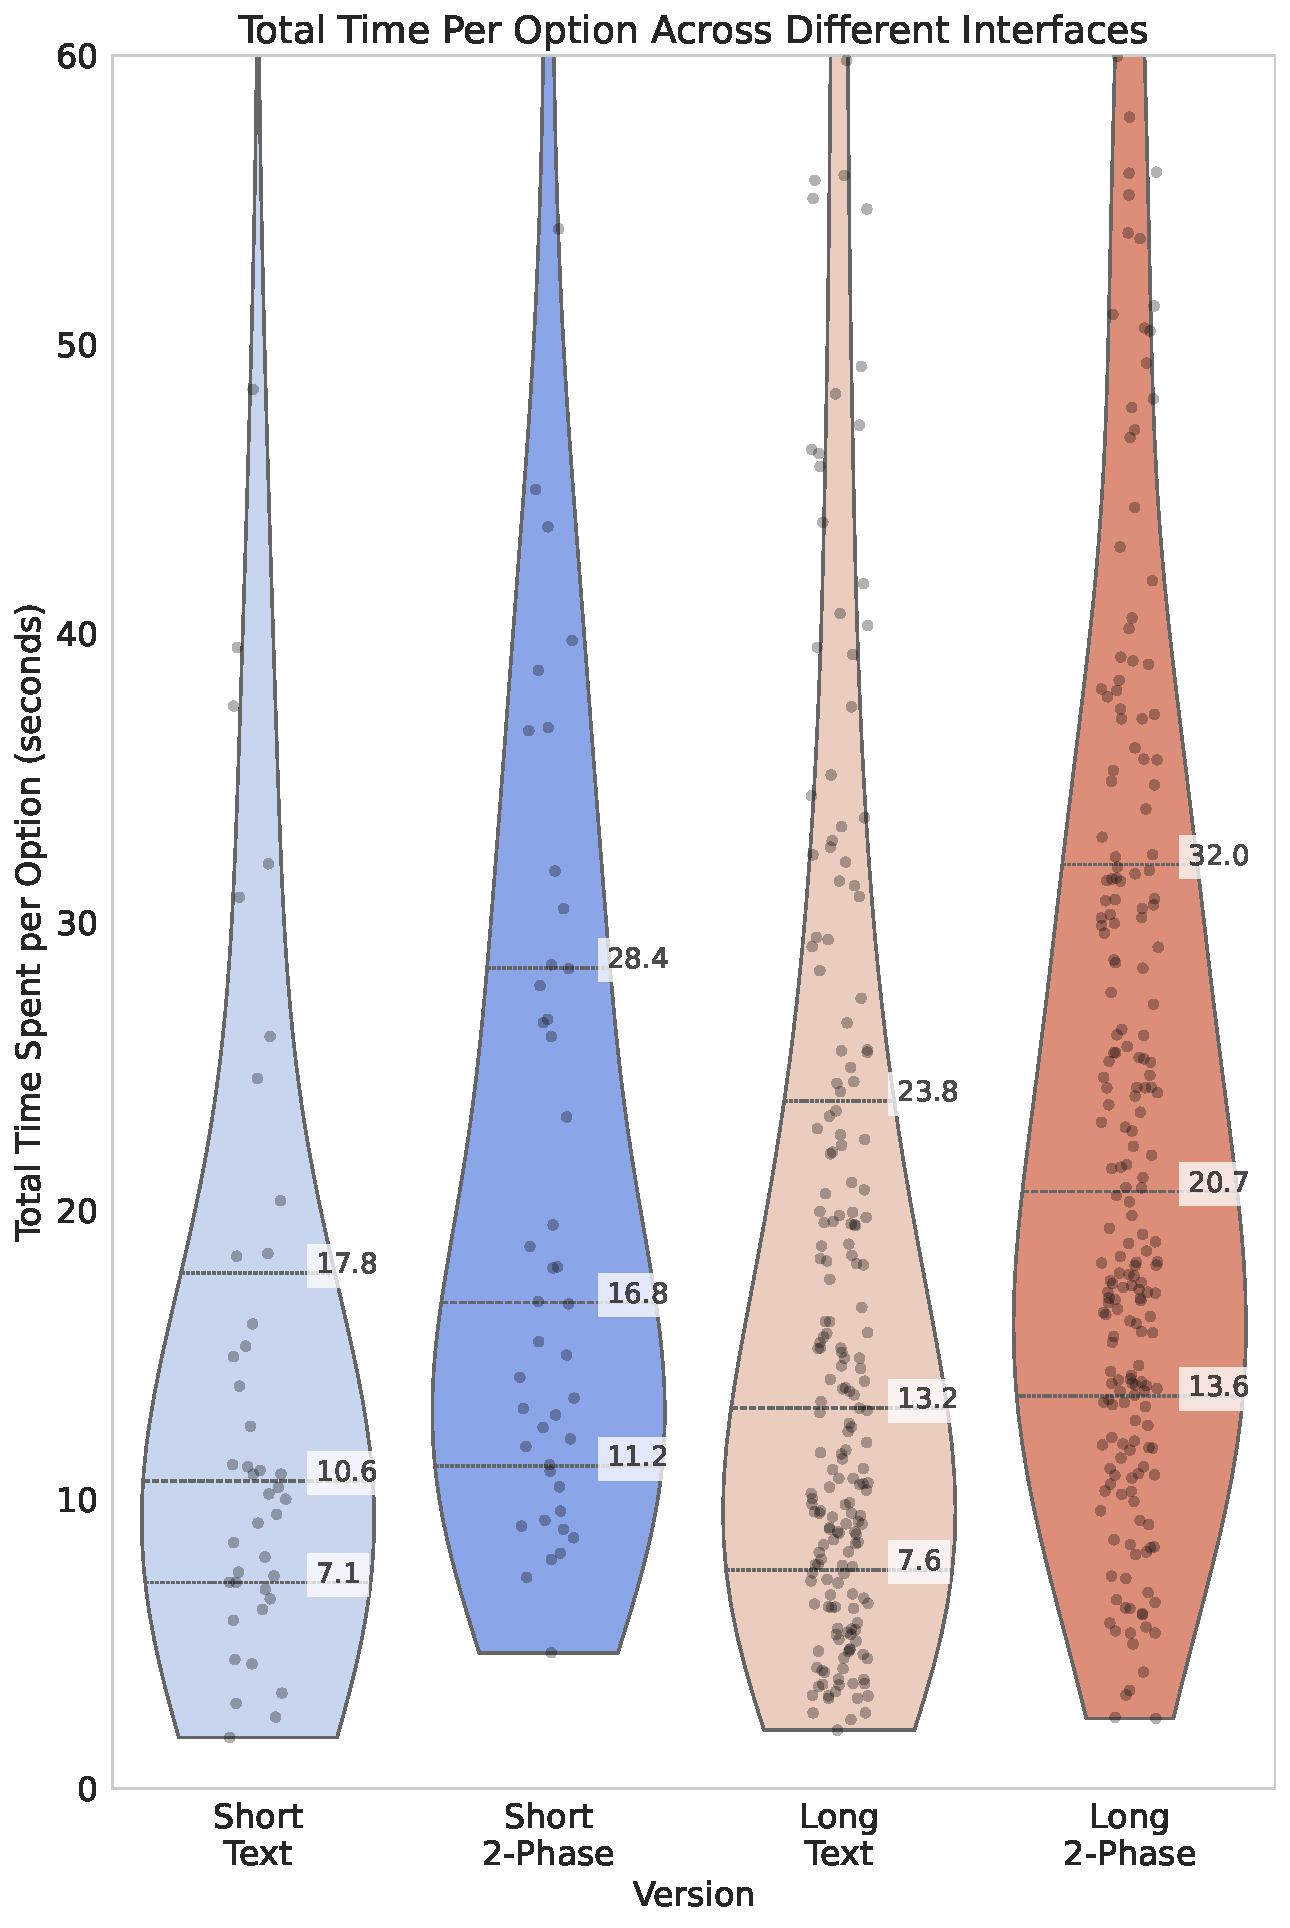
\includegraphics[width=\textwidth]{content/image/results/total_time_per_option.pdf}
            \caption{Total Time per option}
            \label{fig:total_time}
        \end{subfigure}
        \hfill
        \begin{subfigure}[b]{0.26\pdfpageheight}
            \centering
            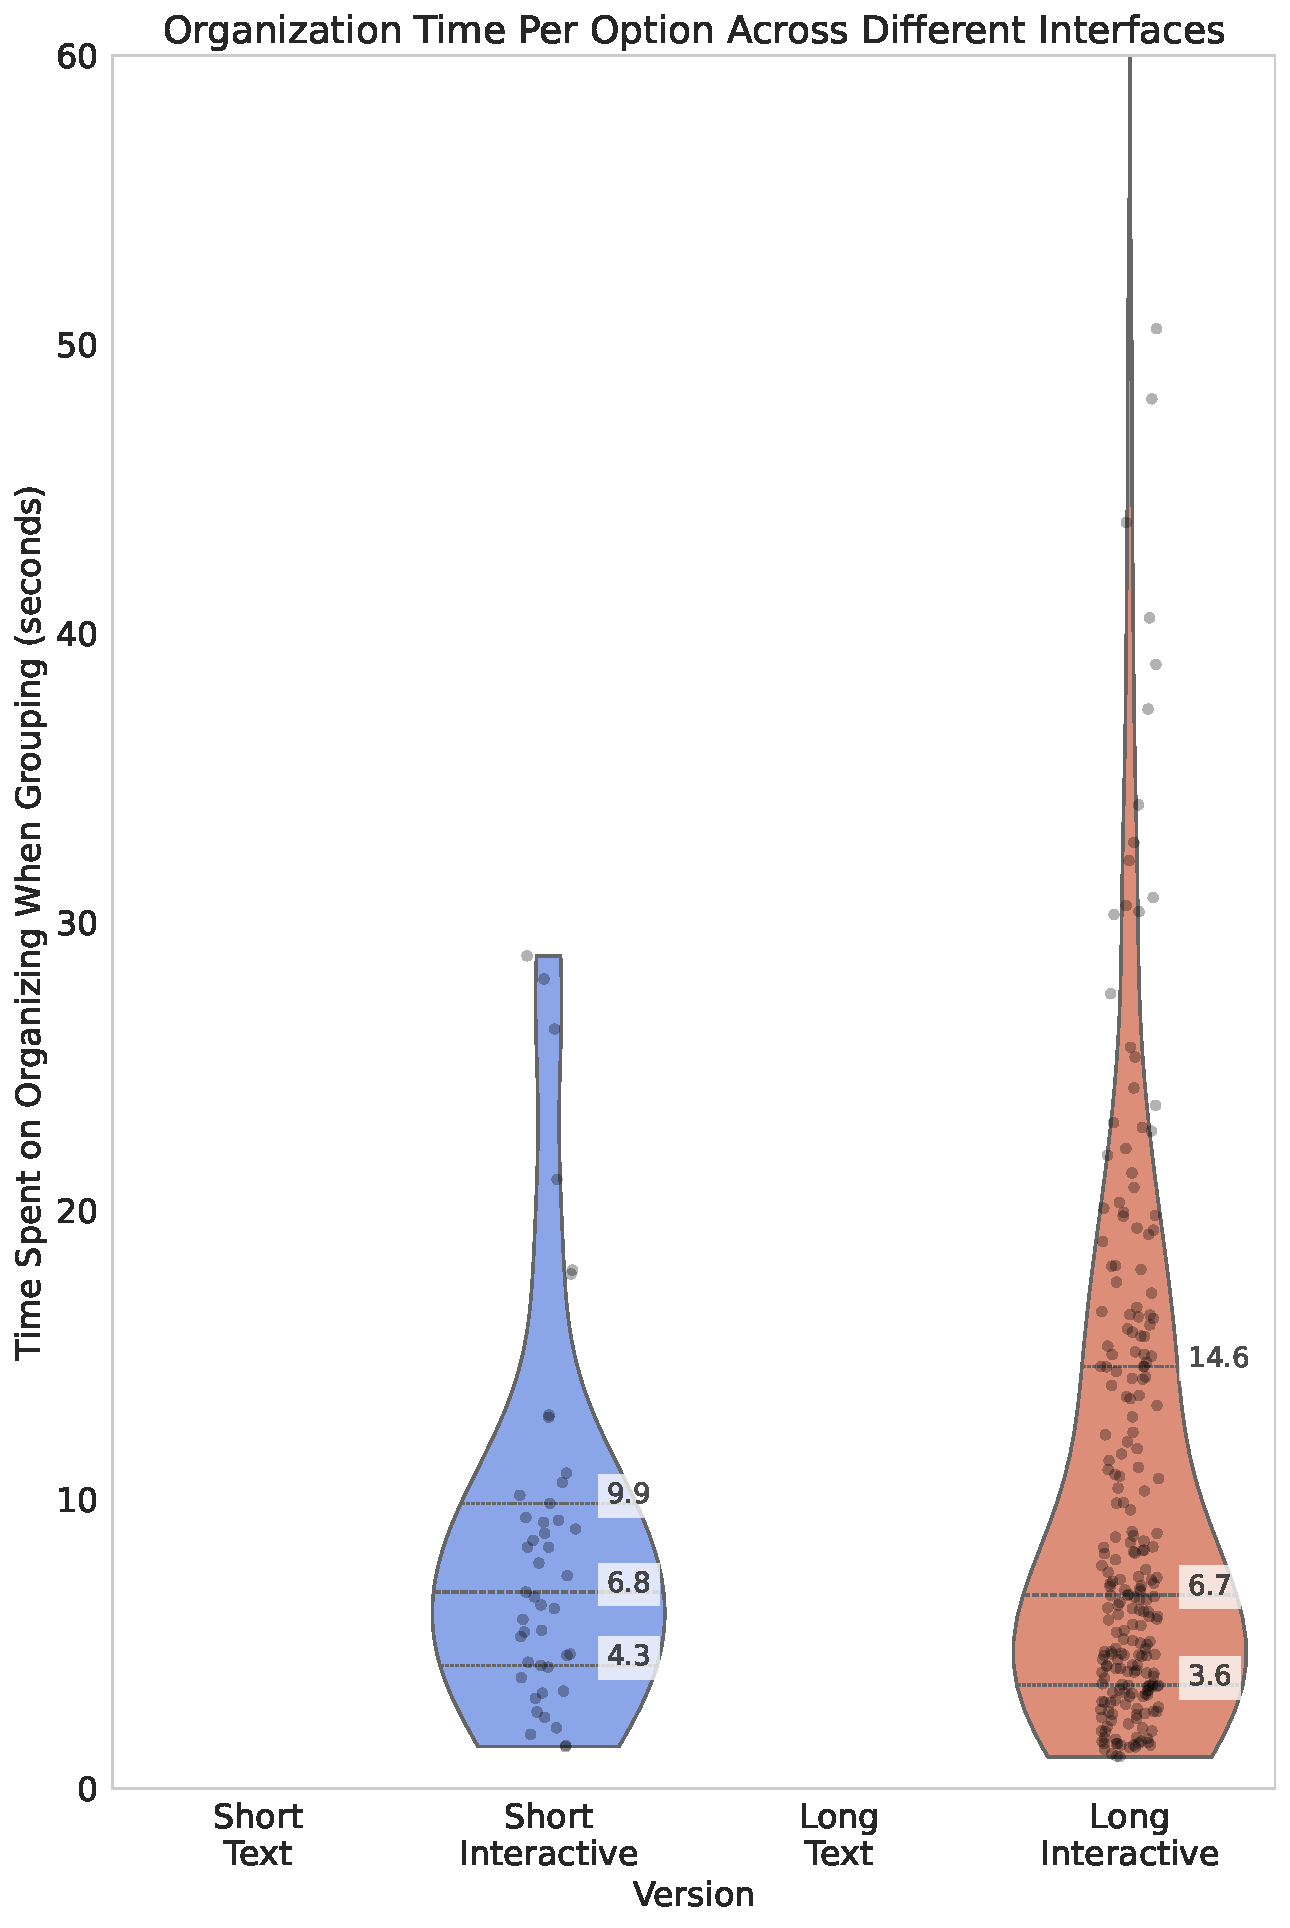
\includegraphics[width=\textwidth]{content/image/results/org_time_per_option.pdf}
            \caption{Organization Time per option}
            \label{fig:org_time}
        \end{subfigure}
        \hfill
        \begin{subfigure}[b]{0.26\pdfpageheight}
            \centering
            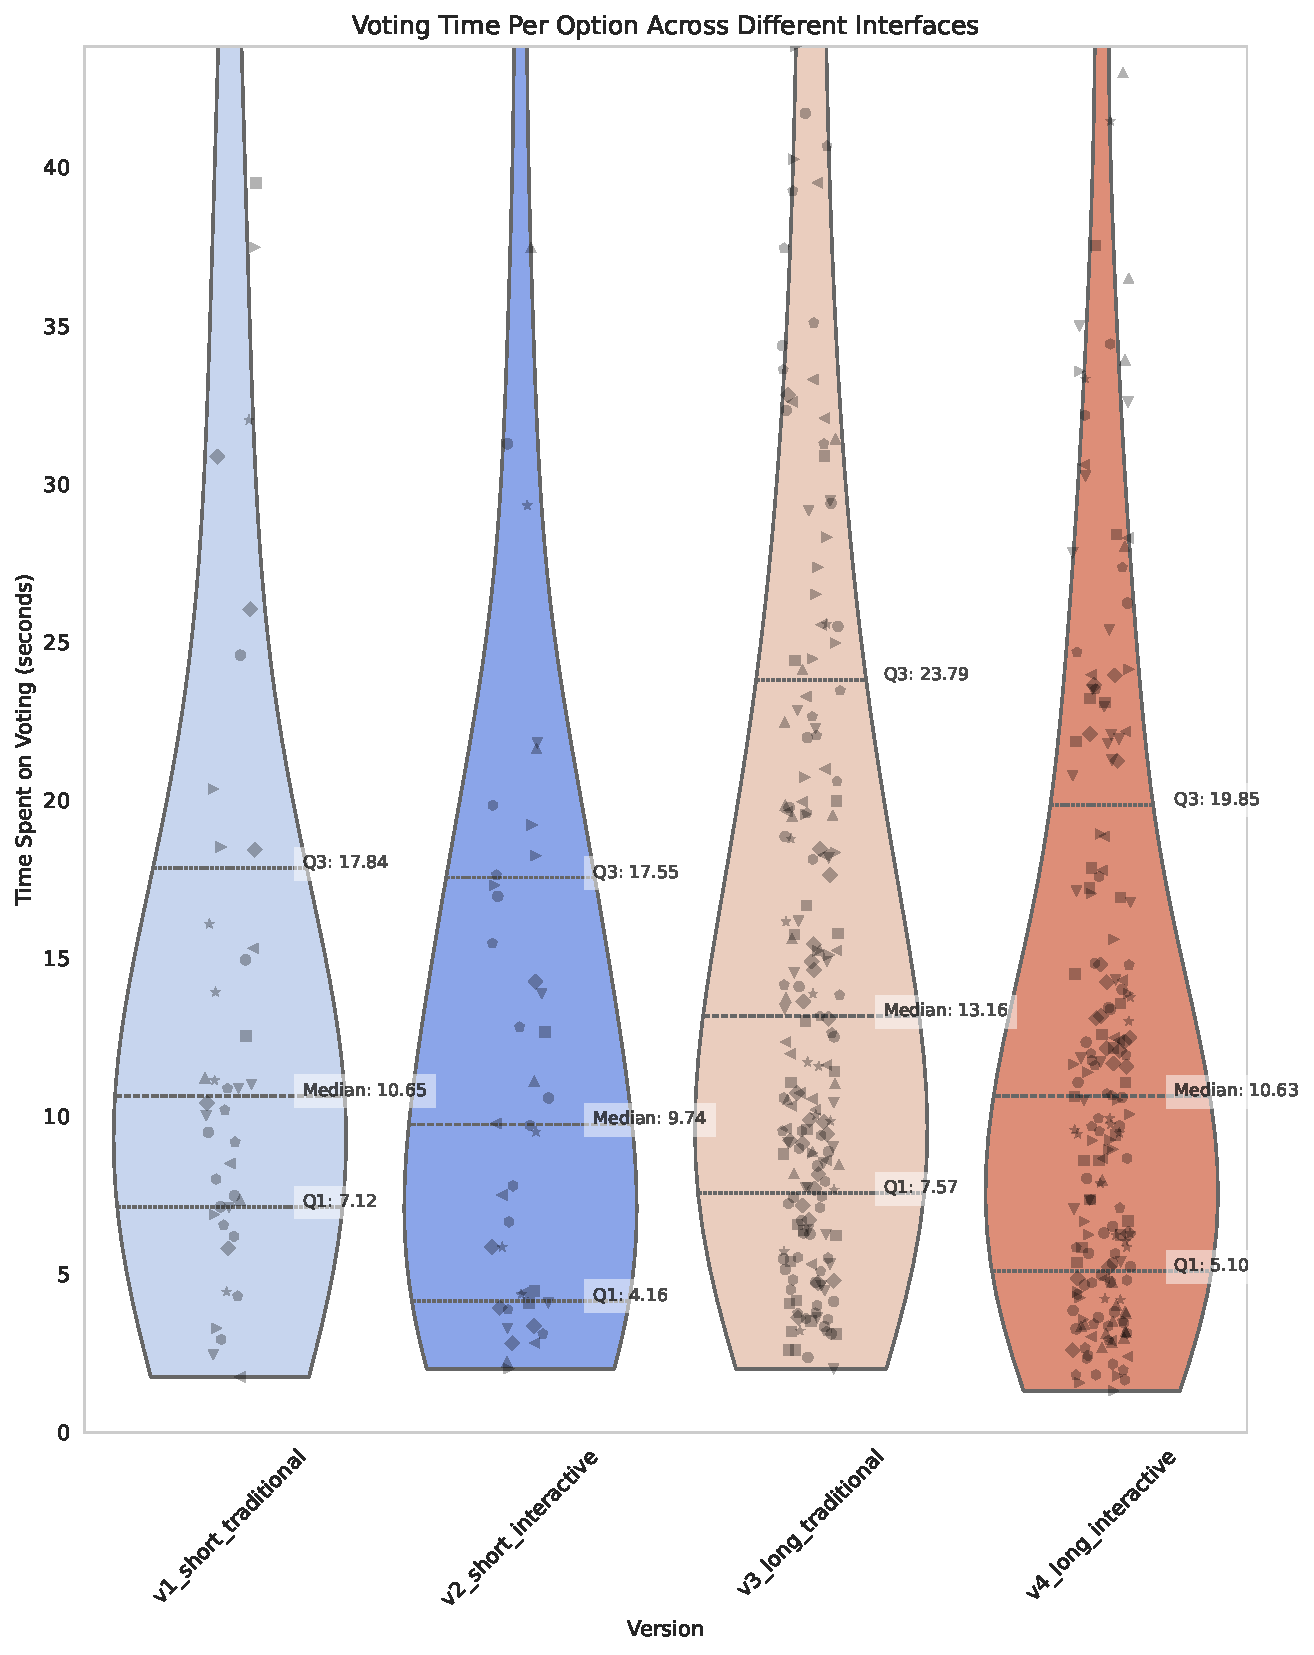
\includegraphics[width=\textwidth]{content/image/results/voting_time_per_option.pdf}
            \caption{Voting Time per option}
            \label{fig:vote_time}
        \end{subfigure}
        \caption{Breakdown of time per option}
        \label{fig:Time Spent Per Option Per Person}
    \end{figure}
\end{landscape}
}

\subsection{Interaction Behavior Analysis}
\label{sec:act}
To answer RQ3 and collect evidence of shifts in participants' cognitive sources, we analyze their behaviors during the survey. We aim to understand the time participants spend on options and when they make changes. When a participant clicks their mouse on the interface to complete an action, such as drag-and-drop, updating votes, or placing options into a specific group, a timestamp and the payload of the update are stored in the log. In this subsection, we analyze these log data. We acknowledge that the time difference between two actions indicates the time the participant took to decide and act. Although participants might be thinking about other things, this is our best proxy to study their behaviors.


\subsection{Time Spent per Options}
First, we define time spent per option. A participant can enact several actions related to the same option, for example, a participant might spend $t_1$ time to place the option into a `lean positive' category; spend $t_2$ and $t_3$ time to drag and drop the options to reposition it on the interactive interface; spend $t_4$ and $t_5$ time to update the upvotes on that option. In this case, we would define voting time as $t_4 + t_5$ for that option, and organization time as $t_1 + t_2 + t_3$.
\hs{I don't understand how each time corresponds to each type of action. Rewrite with action ($t_1$), action ($t_2$) etc.}

To reduce noise, we intentionally drop all the time participants spent on the first option in the organization phase or voting phase. The goal is to reduce the inclusion of time they spent on reading the prompt, forming their preference, or understanding the interface. We present the results in Figure~\ref{fig:Time Spent Per Option Per Person} where each of the dots represents the time accumulated for an option that a participant interacted with. The violin plot shows the distribution of the dots and the three horizontal lines represent the median, 25th percentile, and 75th percentile of the time spent for that interface.

In Figure~\ref{fig:total_time}, we observe that participants spent more time on the interactive interface than the text interface in both short and long surveys. A non-parametric statistical test supports such observation with $p<0.01$ for short and $p<0.0001$ for long surveys. \hs{I'm skeptical of this result; the ranges between Q1 and Q3 across the plots shows quite a bit overalp; what test is this?\\What is interesing in your figure 13(b) is that organization time per option remains the same despite the increased number of options; I would have predicted a slight increase because there are more things to organize; perhaps something to highlight as a benefit of the two stage organizational schema.} \tc{RE:Mann-Whitney U test. So comparing v1 and v2; v3 and v4.} This is not surprising because participants need to review the options and organize them in the interactive interface which takes more time. We break down the total time spent into organization time and voting time in Figure~\ref{fig:org_time} and Figure~\ref{fig:vote_time}.

Once we separate the organization time (Figure~\ref{fig:org_time}) and identify the voting time (Figure~\ref{fig:vote_time}), while there are no statistically significant differences between the text interface and the interactive interface in the short survey, we see a statistically significant reduction ($p<0.01$) in voting time between the text interface and the interactive interface. In other words, our original hypothesis holds in which the two-step design process did facilitate participants in making their decisions.

\begin{figure}[ht]
    \centering
    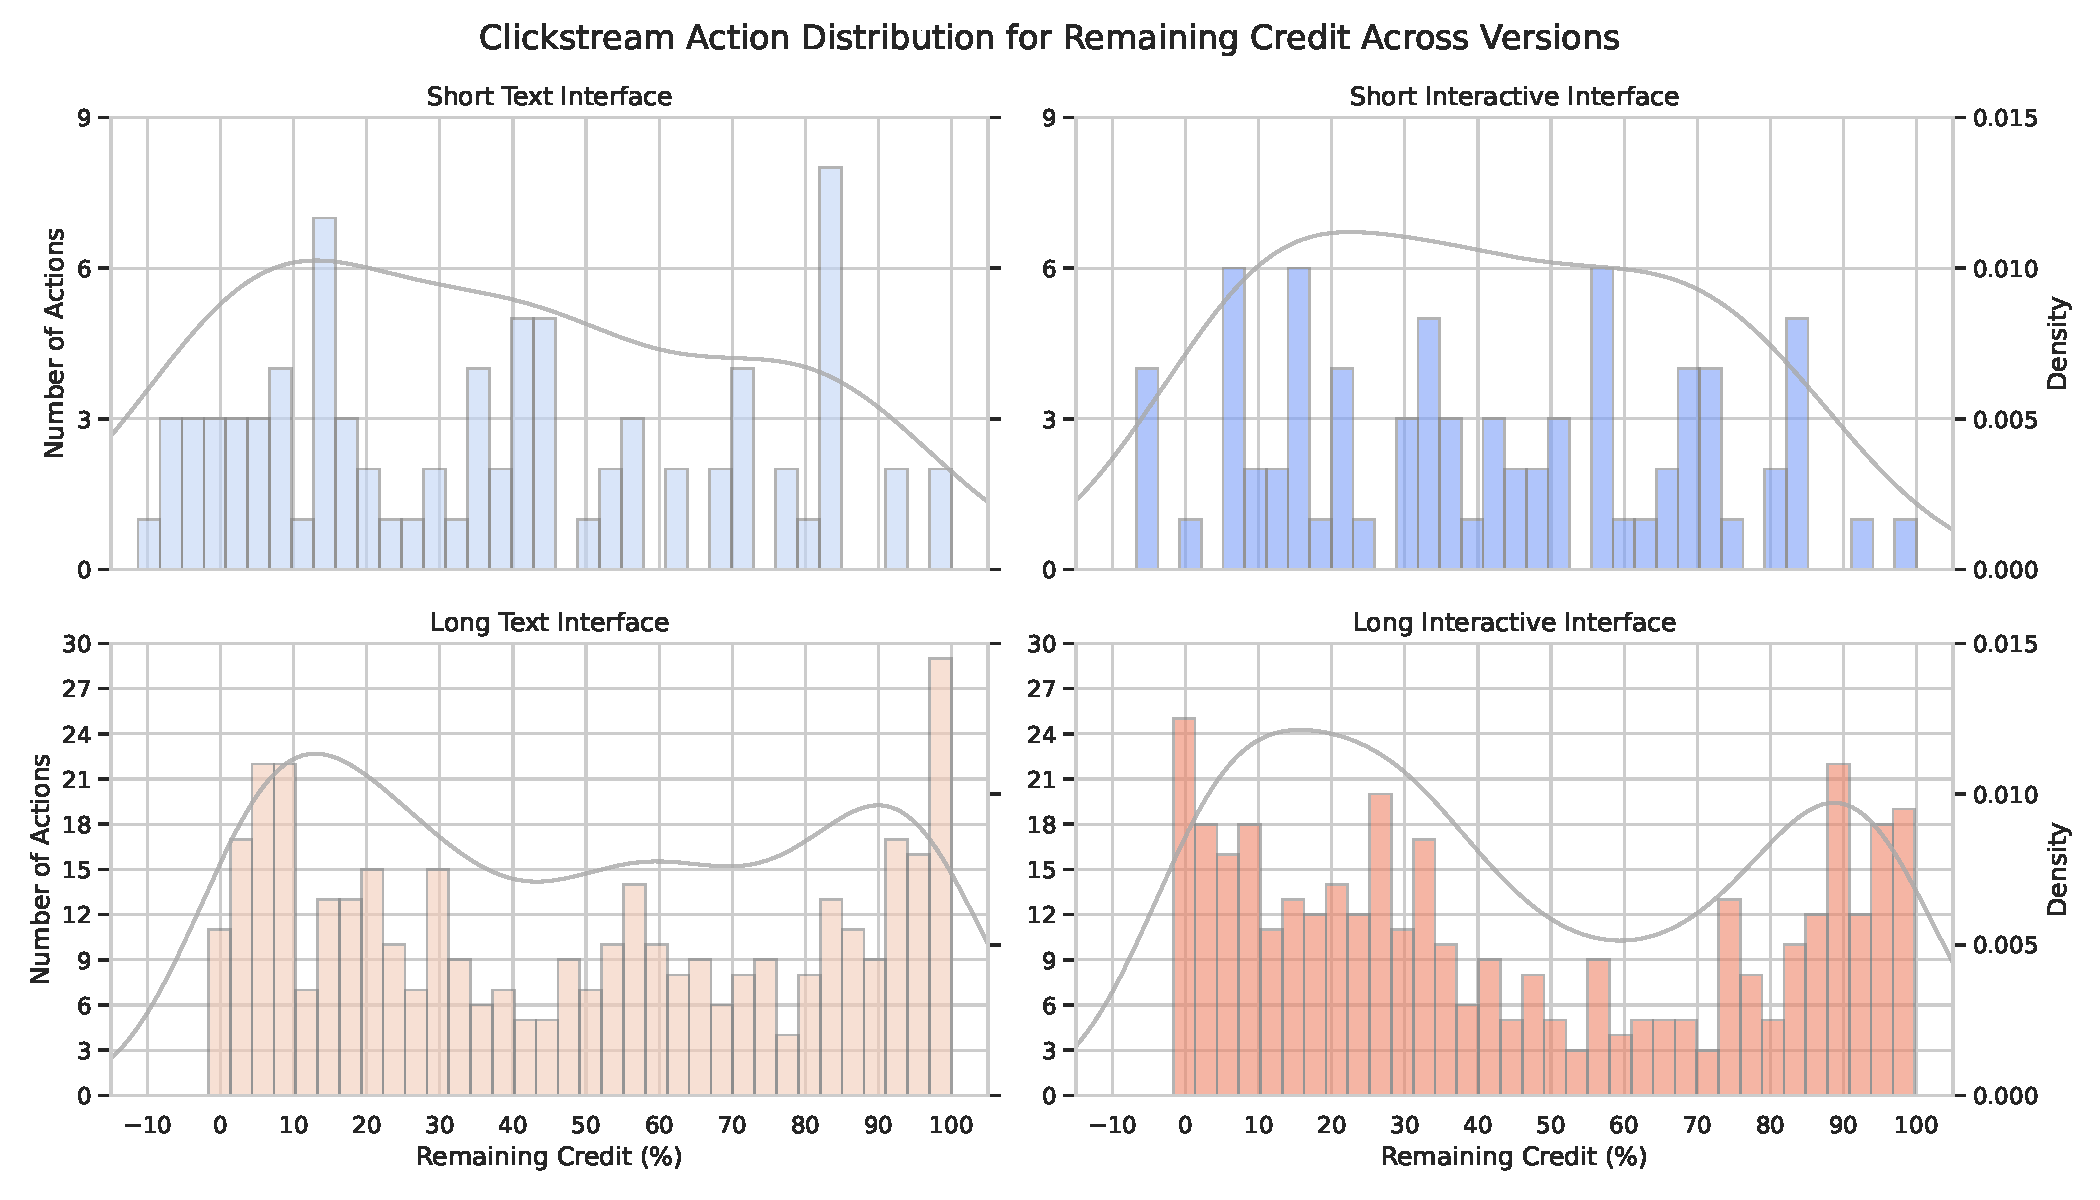
\includegraphics[width=\textwidth]{content/image/results/clickstream_action_distribution.pdf}
    \caption{voting actions across all options (needs to update chart text, remove normalization, and change the dot colors.)}
    \label{fig:voting_all}
\end{figure}

\subsection{Budget and Voting Behaviors}
Next, we examine participants' voting behavior and how it changed throughout the progress. Given that we observe significant differences in voting time changes comparing text interface and interactive interface for the long option survey, we focus on deciphering the voting action changes between these two experiment conditions in this subsection.

Figure~\ref{fig:voting_all} plots the time of voting actions over the remainder of the participant's budget across the text and interactive interface across all four groups. In other words, different from~\textcite{quarfoot2017quadratic} focusing on the number of accumulated votes over an individual's time, where they showed QV voters make more revisions than Likert Surveys, we focused on the budget scarcity which can influence QS respondents' behaviors.

In this plot, we see two distinct patterns between the short survey and the long survey in terms of participant behaviors. Only in the long surveys did participants exhibit more actions when the budget was abundant and when it began to run out, with the long interactive interface being more significant.

\begin{figure}[ht]
    \centering
    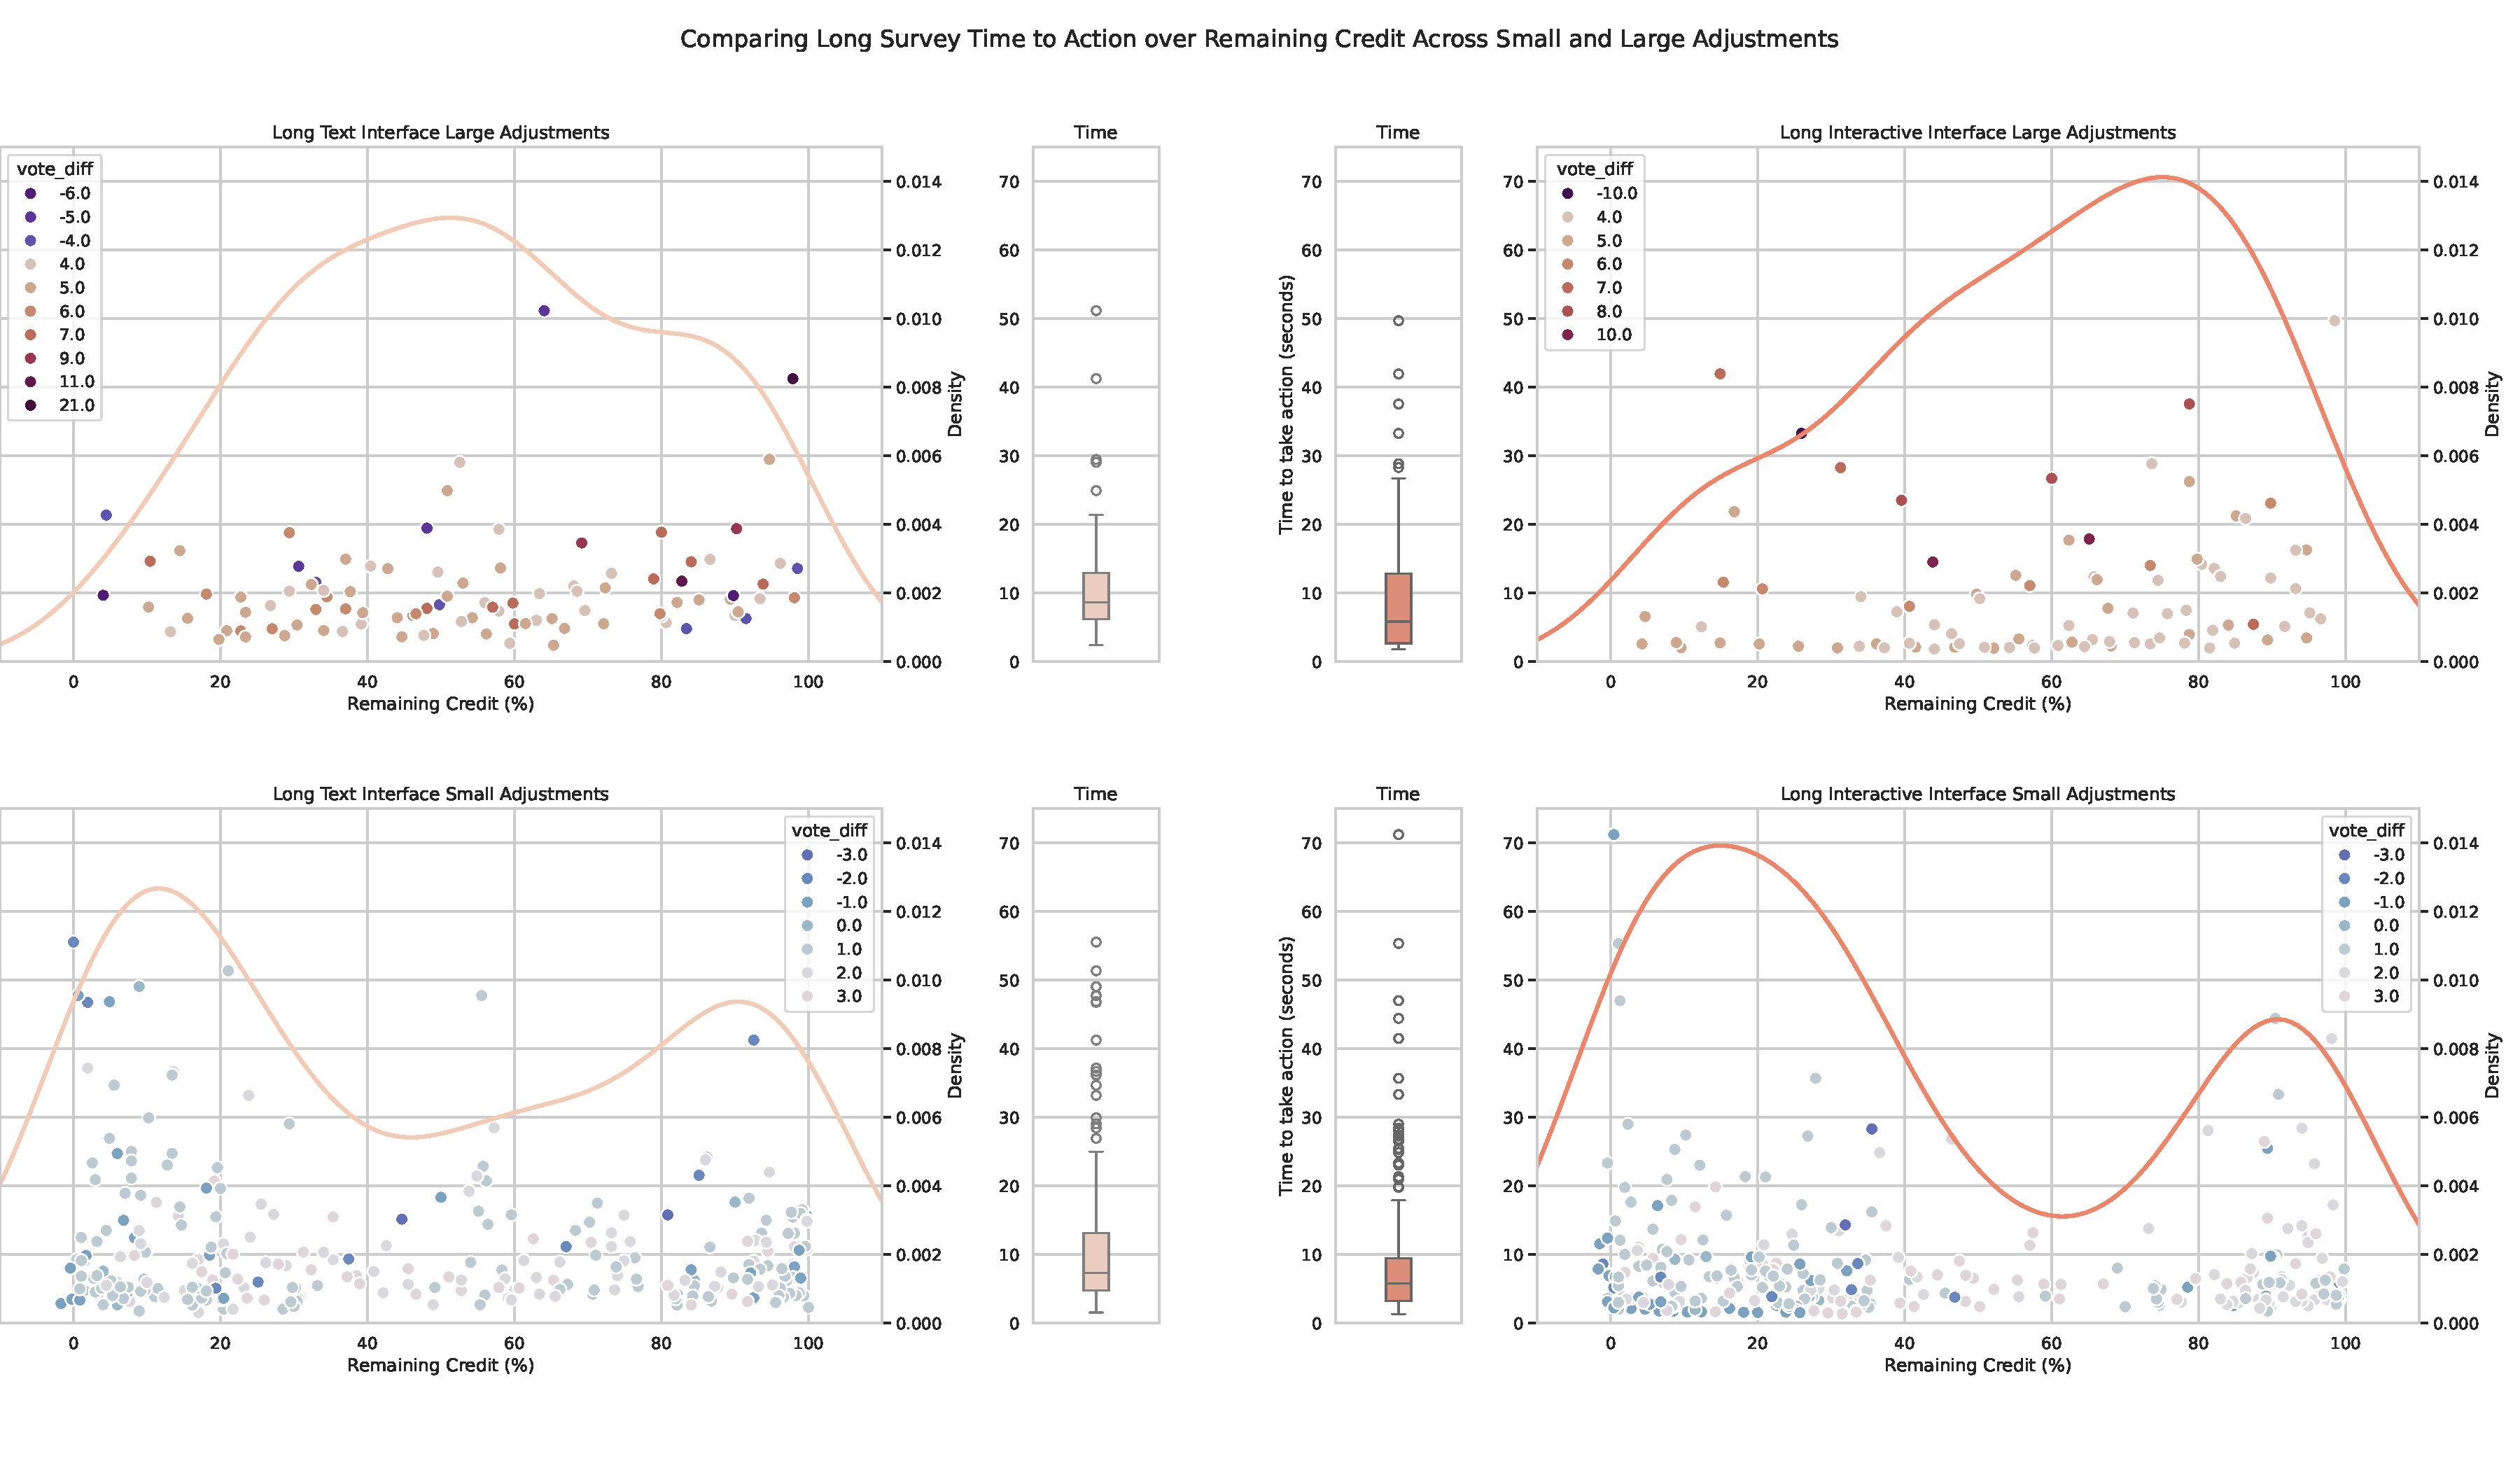
\includegraphics[width=\textwidth]{content/image/results/combined_density_plots.pdf}
    \caption{Breakdown of voting actions (needs to update chart text)}
    \label{fig:voting_v3_v4}
\end{figure}

Thus, we further separated the behaviors where participants made bigger changes or smaller changes to the option, specifically for the long version. In Figure~\ref{fig:voting_v3_v4} , we define an adjustment of four or more votes as a large adjustment which we plotted in the first row of the Figure. Adjustments of three or fewer votes are considered small adjustments.\hs{how do you justify this?}

First, we are able to surface the bimodal action distribution in both plots, with a even stronger signal for long interactive interface participants. Second, the plot demonstrated a clear cluster of voting actions in the bottom left corner of the interactive interface for small vote adjustments. In other words, participants made much smaller but more rapid adjustments when their budgets were running low. Second, larger adjustments are made when the participants have more options comparing the two plots on the first row. We interpret this behavior as participants in the interactive interface have constructed a clearer image of option preferences and, hence, have the ability to take larger strides in allotting their budget and deciding the number of votes at the beginning of the survey. Toward the end, participants using the interactive interface are then making fine-tuned adjustments to ensure that their preferences are reflected in their submissions.

% add qualitative support
\paragraph{Iterative Support from Interactive Interface}
\hs{this para seems out of place; perhaps should be merged with next section?}
Among all the interviews, when discussing about their experience of the interface, five particpants pointed out the importance of flexibility on the interface and how they took an incremental and iterative approach to navigating their attitude expression. All these participants are using the interactive interface. While this does not mean the study participant using the text interface did not use an iterative approach, but this highlighted the interactive interface encouraged the participants to make iterative and incremental updates. As one participant pointed out:

\begin{displayquote}
I like the fact that it remembers everything that you know. If if you make a mistake, that you don't lose all the work that you've already done. so I think that's very important is that it's an iterative process.

\noindent \hfill -- S019, long interactive interface.
\end{displayquote}

% Ti-Chung Cheng: So what elements of the software interface do you dislike, or like the most, if any, when expressing your preferences on responding to societal issues?
% S009: Hmm! What I like the most actually, probably the sorting function. I think that it really helped me organize my thoughts really, clearly, in terms of what I would dislike the most. really, not that much. I would say. yeah, also, like how we could categorize it, like even within the voting stage rather than just at the categorization stage. 

% Ti-Chung Cheng: Can you tell me a little bit more about the screen? How did the vertical screen help you?
% S037: I think because it helps the layout of, because it's like a long 3 bar. So it's easier for you to to drag and drop, and you can actually sort it, judging by the votes. But I do not do that. But I think this layout is could be helpful in that aspect.

